Посмотрим на поведение характеристик при фиксированных параметрах построения графов для распределения Лапласа и косого нормального, с варьирующимися параметрами распределений. Ниже графики, на которых перебираются различные параметры $\alpha_{laplace}, \beta_{laplace}, \alpha_{skew}$ при фиксированных параметрах графа:
\begin{itemize}
    \item Размер графа =  40
    \item K в KNN = 3
    \item dist в Distance = 1
    \item характеристика для KNN графа - число треугольников (на этой странице)
    \item характеристика для Dist графа - максимальное независимое множество
\end{itemize}
\\

\hspace*{-1cm}
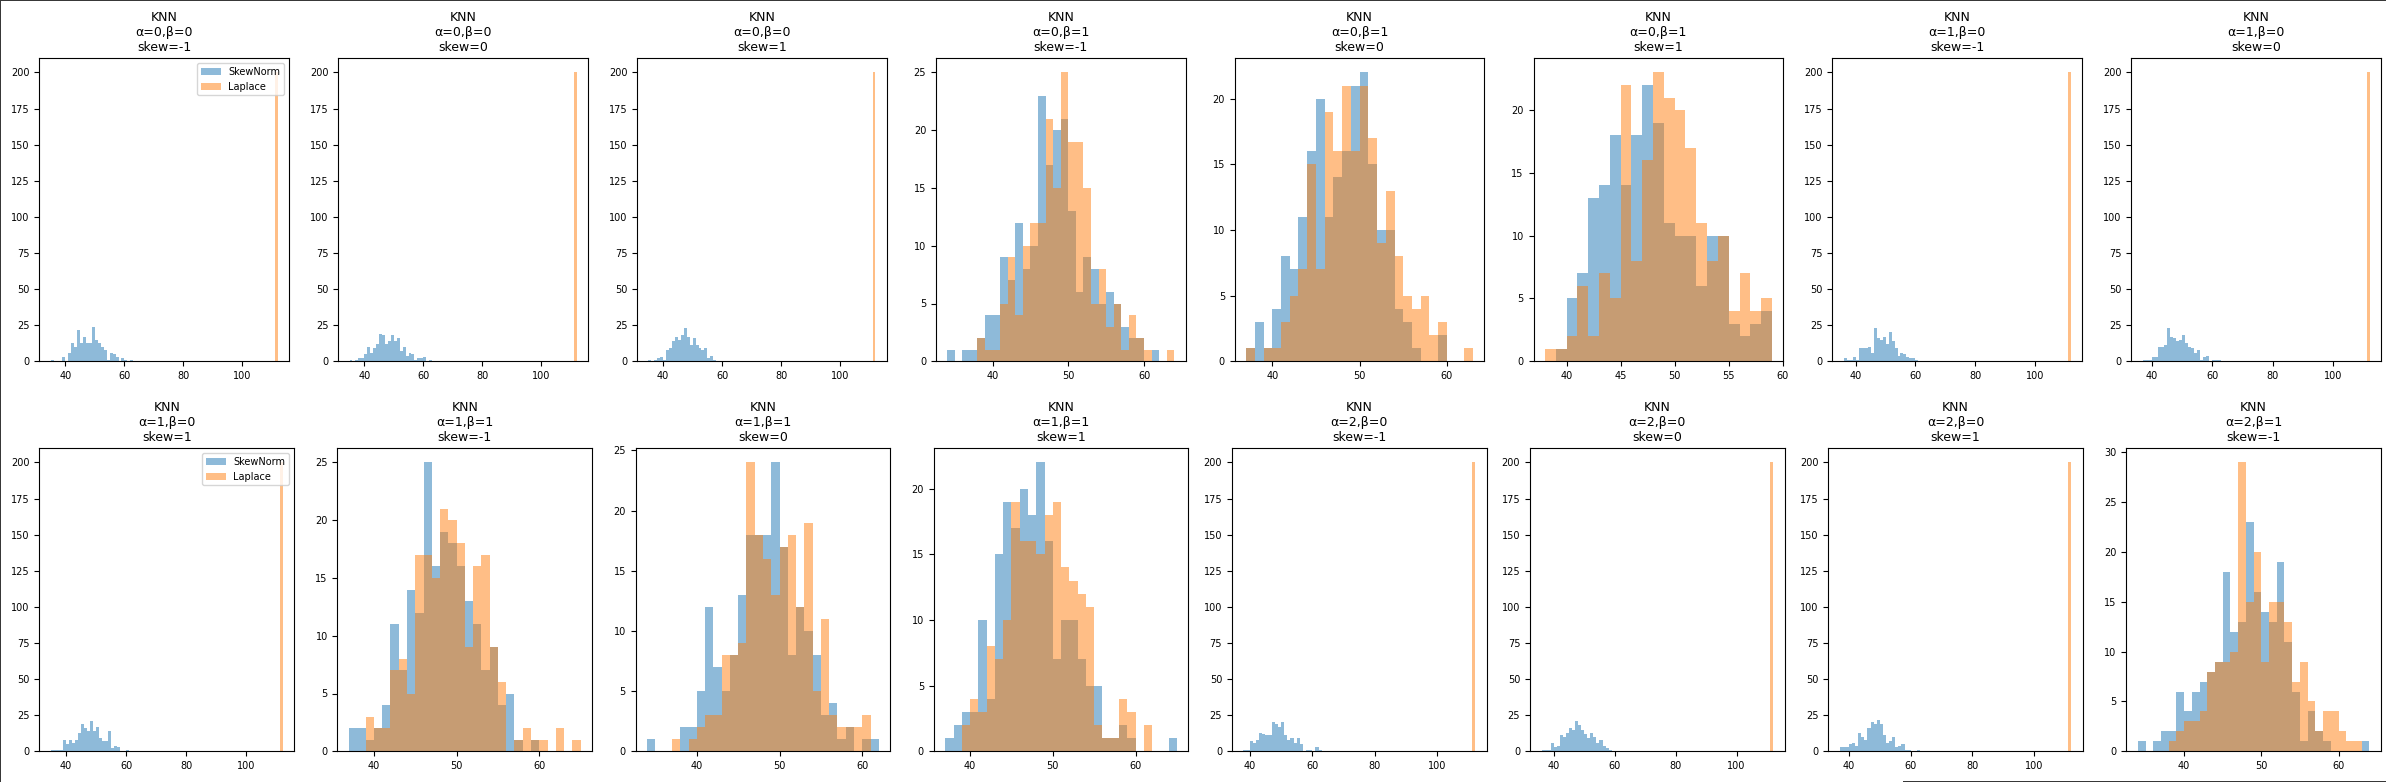
\includegraphics[width=1\textwidth]{Part-I-Ivanova/1_hist.png}\\ 
\hspace*{-0.5cm}
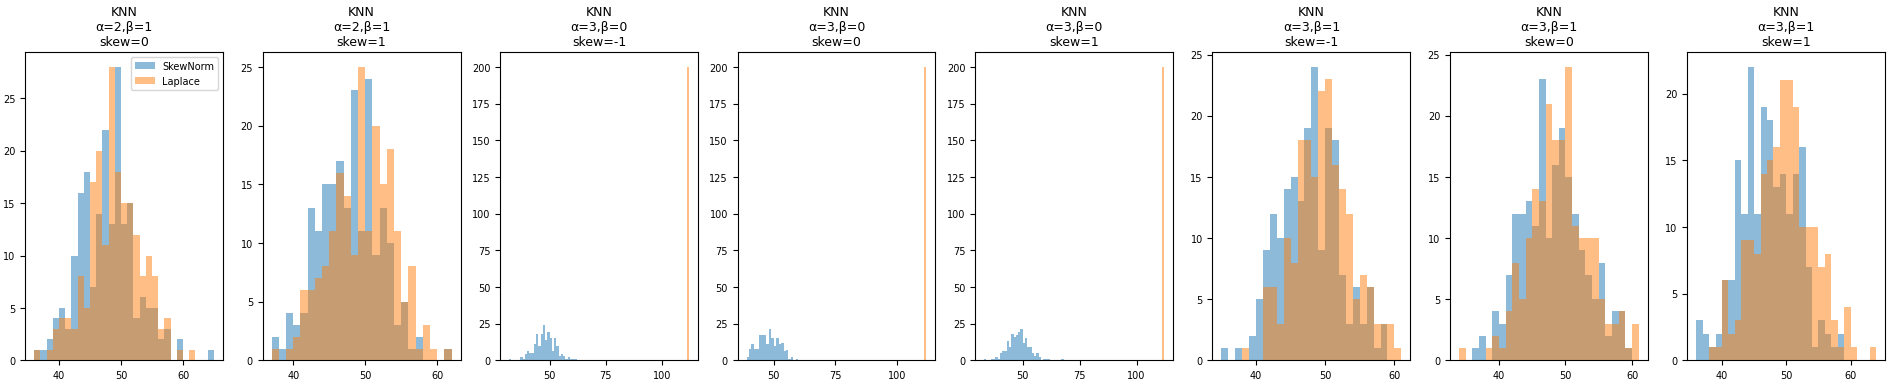
\includegraphics[width=1\textwidth]{Part-I-Ivanova/4_hist.png}\\ 
\textbf{Вывод:} в зависимости от параметров распределений характеристика 'Количество треугольников' KNN графа может быть \textbf{очень хорошим} признаком классификации при хороших параметрах распределений, а при некоторых графики практически идентичны, распределения трудно отличимы.
\newpage
\noindent\textbf{Далее графики для дистанционного графа :} \\\\


\hspace*{-1cm}
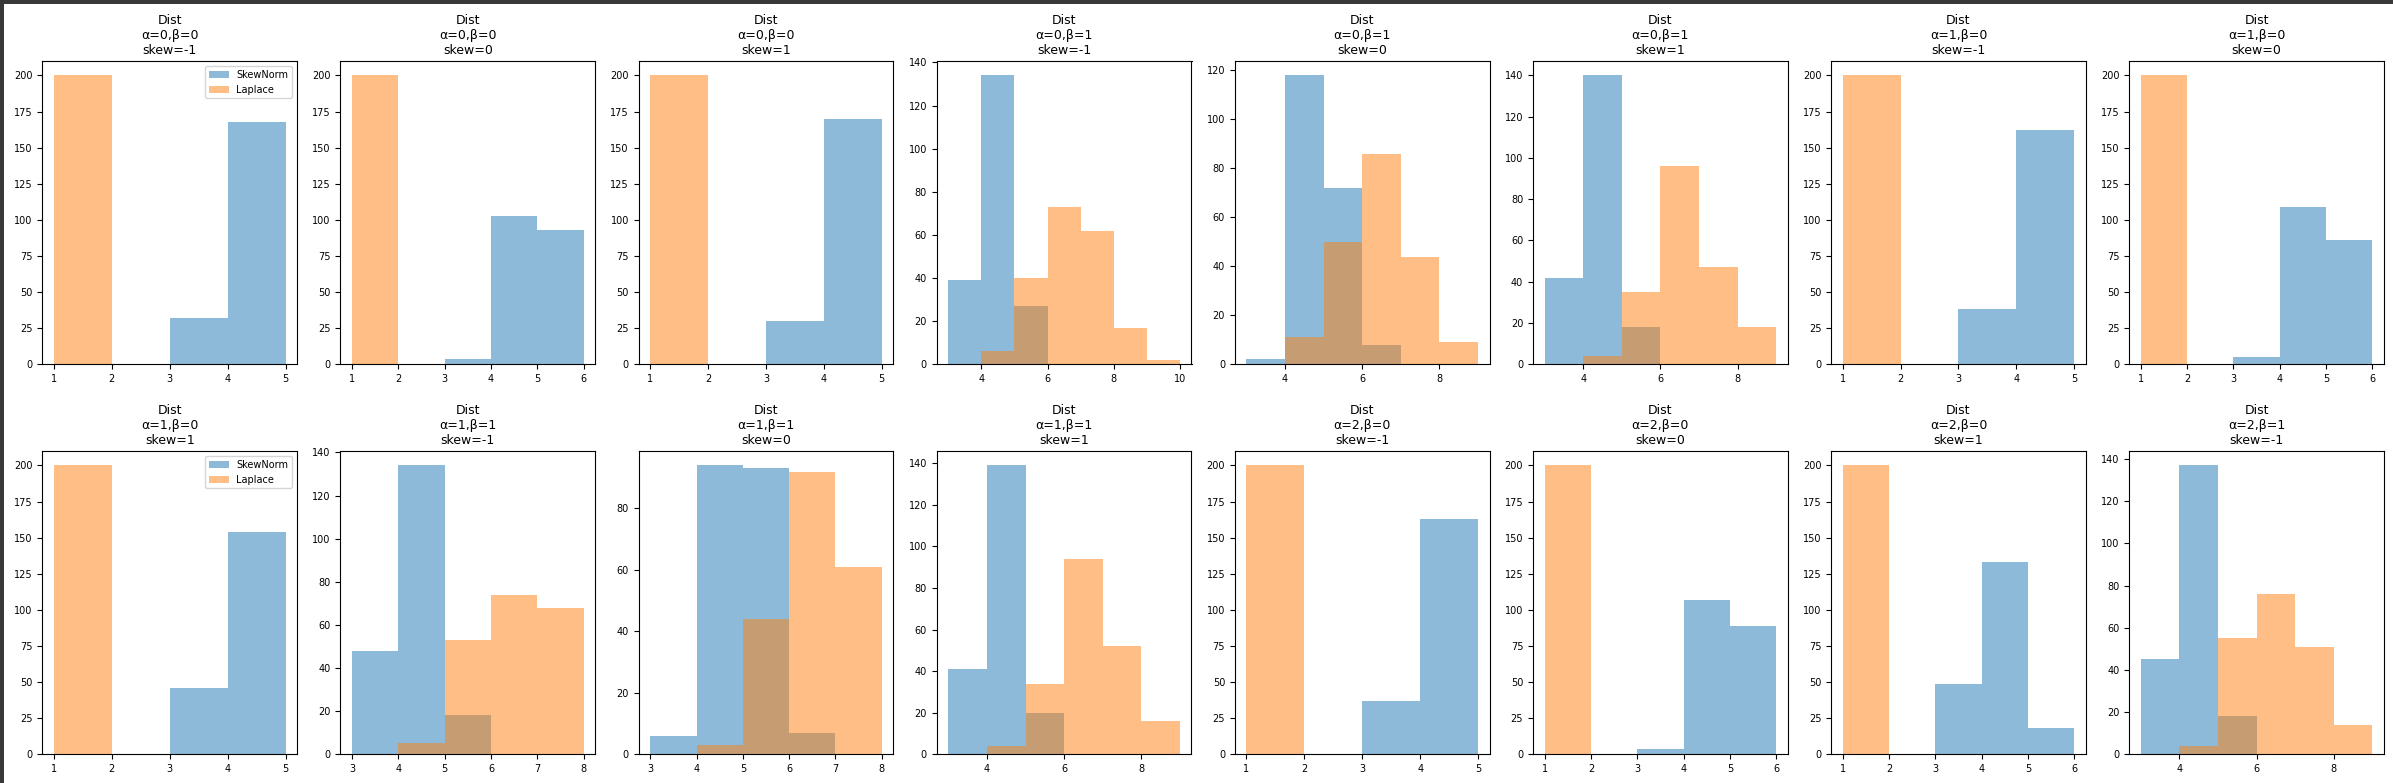
\includegraphics[width=1\textwidth]{Part-I-Ivanova/2_hist.png}
\\
\hspace*{-0.5cm}
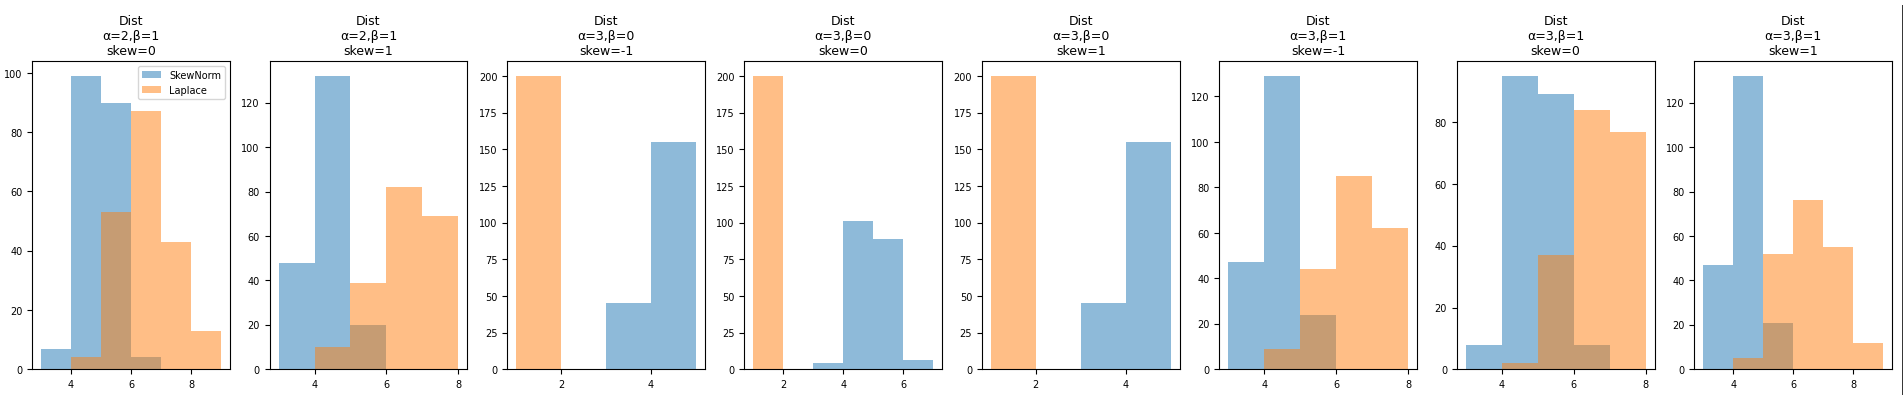
\includegraphics[width=1\textwidth]{Part-I-Ivanova/3_hist.png}\\ 


\noindent\textbf{Вывод:} в целом характеристика 'Размер максимального независимого множества' неплохая характеристика, при некоторых параметрах она лучше разделяет распределения, в некоторых хуже, но в целом всегда неплохо.
